% Options for packages loaded elsewhere
\PassOptionsToPackage{unicode}{hyperref}
\PassOptionsToPackage{hyphens}{url}
%
\documentclass[
  man]{apa6}
\usepackage{amsmath,amssymb}
\usepackage{iftex}
\ifPDFTeX
  \usepackage[T1]{fontenc}
  \usepackage[utf8]{inputenc}
  \usepackage{textcomp} % provide euro and other symbols
\else % if luatex or xetex
  \usepackage{unicode-math} % this also loads fontspec
  \defaultfontfeatures{Scale=MatchLowercase}
  \defaultfontfeatures[\rmfamily]{Ligatures=TeX,Scale=1}
\fi
\usepackage{lmodern}
\ifPDFTeX\else
  % xetex/luatex font selection
\fi
% Use upquote if available, for straight quotes in verbatim environments
\IfFileExists{upquote.sty}{\usepackage{upquote}}{}
\IfFileExists{microtype.sty}{% use microtype if available
  \usepackage[]{microtype}
  \UseMicrotypeSet[protrusion]{basicmath} % disable protrusion for tt fonts
}{}
\makeatletter
\@ifundefined{KOMAClassName}{% if non-KOMA class
  \IfFileExists{parskip.sty}{%
    \usepackage{parskip}
  }{% else
    \setlength{\parindent}{0pt}
    \setlength{\parskip}{6pt plus 2pt minus 1pt}}
}{% if KOMA class
  \KOMAoptions{parskip=half}}
\makeatother
\usepackage{xcolor}
\usepackage{longtable,booktabs,array}
\usepackage{calc} % for calculating minipage widths
% Correct order of tables after \paragraph or \subparagraph
\usepackage{etoolbox}
\makeatletter
\patchcmd\longtable{\par}{\if@noskipsec\mbox{}\fi\par}{}{}
\makeatother
% Allow footnotes in longtable head/foot
\IfFileExists{footnotehyper.sty}{\usepackage{footnotehyper}}{\usepackage{footnote}}
\makesavenoteenv{longtable}
\usepackage{graphicx}
\makeatletter
\def\maxwidth{\ifdim\Gin@nat@width>\linewidth\linewidth\else\Gin@nat@width\fi}
\def\maxheight{\ifdim\Gin@nat@height>\textheight\textheight\else\Gin@nat@height\fi}
\makeatother
% Scale images if necessary, so that they will not overflow the page
% margins by default, and it is still possible to overwrite the defaults
% using explicit options in \includegraphics[width, height, ...]{}
\setkeys{Gin}{width=\maxwidth,height=\maxheight,keepaspectratio}
% Set default figure placement to htbp
\makeatletter
\def\fps@figure{htbp}
\makeatother
\setlength{\emergencystretch}{3em} % prevent overfull lines
\providecommand{\tightlist}{%
  \setlength{\itemsep}{0pt}\setlength{\parskip}{0pt}}
\setcounter{secnumdepth}{-\maxdimen} % remove section numbering
% Make \paragraph and \subparagraph free-standing
\ifx\paragraph\undefined\else
  \let\oldparagraph\paragraph
  \renewcommand{\paragraph}[1]{\oldparagraph{#1}\mbox{}}
\fi
\ifx\subparagraph\undefined\else
  \let\oldsubparagraph\subparagraph
  \renewcommand{\subparagraph}[1]{\oldsubparagraph{#1}\mbox{}}
\fi
\ifLuaTeX
\usepackage[bidi=basic]{babel}
\else
\usepackage[bidi=default]{babel}
\fi
\babelprovide[main,import]{english}
% get rid of language-specific shorthands (see #6817):
\let\LanguageShortHands\languageshorthands
\def\languageshorthands#1{}
% Manuscript styling
\usepackage{upgreek}
\captionsetup{font=singlespacing,justification=justified}

% Table formatting
\usepackage{longtable}
\usepackage{lscape}
% \usepackage[counterclockwise]{rotating}   % Landscape page setup for large tables
\usepackage{multirow}		% Table styling
\usepackage{tabularx}		% Control Column width
\usepackage[flushleft]{threeparttable}	% Allows for three part tables with a specified notes section
\usepackage{threeparttablex}            % Lets threeparttable work with longtable

% Create new environments so endfloat can handle them
% \newenvironment{ltable}
%   {\begin{landscape}\centering\begin{threeparttable}}
%   {\end{threeparttable}\end{landscape}}
\newenvironment{lltable}{\begin{landscape}\centering\begin{ThreePartTable}}{\end{ThreePartTable}\end{landscape}}

% Enables adjusting longtable caption width to table width
% Solution found at http://golatex.de/longtable-mit-caption-so-breit-wie-die-tabelle-t15767.html
\makeatletter
\newcommand\LastLTentrywidth{1em}
\newlength\longtablewidth
\setlength{\longtablewidth}{1in}
\newcommand{\getlongtablewidth}{\begingroup \ifcsname LT@\roman{LT@tables}\endcsname \global\longtablewidth=0pt \renewcommand{\LT@entry}[2]{\global\advance\longtablewidth by ##2\relax\gdef\LastLTentrywidth{##2}}\@nameuse{LT@\roman{LT@tables}} \fi \endgroup}

% \setlength{\parindent}{0.5in}
% \setlength{\parskip}{0pt plus 0pt minus 0pt}

% Overwrite redefinition of paragraph and subparagraph by the default LaTeX template
% See https://github.com/crsh/papaja/issues/292
\makeatletter
\renewcommand{\paragraph}{\@startsection{paragraph}{4}{\parindent}%
  {0\baselineskip \@plus 0.2ex \@minus 0.2ex}%
  {-1em}%
  {\normalfont\normalsize\bfseries\itshape\typesectitle}}

\renewcommand{\subparagraph}[1]{\@startsection{subparagraph}{5}{1em}%
  {0\baselineskip \@plus 0.2ex \@minus 0.2ex}%
  {-\z@\relax}%
  {\normalfont\normalsize\itshape\hspace{\parindent}{#1}\textit{\addperi}}{\relax}}
\makeatother

% \usepackage{etoolbox}
\makeatletter
\patchcmd{\HyOrg@maketitle}
  {\section{\normalfont\normalsize\abstractname}}
  {\section*{\normalfont\normalsize\abstractname}}
  {}{\typeout{Failed to patch abstract.}}
\patchcmd{\HyOrg@maketitle}
  {\section{\protect\normalfont{\@title}}}
  {\section*{\protect\normalfont{\@title}}}
  {}{\typeout{Failed to patch title.}}
\makeatother

\usepackage{xpatch}
\makeatletter
\xapptocmd\appendix
  {\xapptocmd\section
    {\addcontentsline{toc}{section}{\appendixname\ifoneappendix\else~\theappendix\fi\\: #1}}
    {}{\InnerPatchFailed}%
  }
{}{\PatchFailed}
\DeclareDelayedFloatFlavor{ThreePartTable}{table}
\DeclareDelayedFloatFlavor{lltable}{table}
\DeclareDelayedFloatFlavor*{longtable}{table}
\makeatletter
\renewcommand{\efloat@iwrite}[1]{\immediate\expandafter\protected@write\csname efloat@post#1\endcsname{}}
\makeatother
\usepackage{lineno}

\linenumbers
\usepackage{csquotes}
\ifLuaTeX
  \usepackage{selnolig}  % disable illegal ligatures
\fi
\IfFileExists{bookmark.sty}{\usepackage{bookmark}}{\usepackage{hyperref}}
\IfFileExists{xurl.sty}{\usepackage{xurl}}{} % add URL line breaks if available
\urlstyle{same}
\hypersetup{
  pdftitle={Goodale Consult},
  pdfauthor={Kyle Parrish1},
  pdflang={en-EN},
  hidelinks,
  pdfcreator={LaTeX via pandoc}}

\title{Goodale Consult}
\author{Kyle Parrish\textsuperscript{1}}
\date{}


\shorttitle{Goodale Consult}

\affiliation{\phantom{0}}

\begin{document}
\maketitle

Here are some initial plots and tables that I hope are a good start. I took some notes from the excel sheet and applied them as I understood them to the data. This html format is one of the best for copy-pasting, but I can also provide a pdf or word document.

\hypertarget{what-pitch-accents-tend-to-mark-focus}{%
\subsection{What Pitch Accents tend to mark focus?}\label{what-pitch-accents-tend-to-mark-focus}}

I first created tables to try an answer this question. Each table and figure are comparing pitch accents for the positions ``N'' and ``N1'' in either Broad of Narrow focus in each city (Montevideo or Durazno). I looked back at the spread sheet and may be misunderstanding what is supposed to be focused. If I have chosen the wrong word in the sentence, please just let me know which position and sentence I should make similar visualizations for.

\emph{Broad Focus Declaratives}

I started with Broad focus declaratives (position is ``N''). The table shows the occurance of each pitch accent in the data without cleaning up the very rare cases (under 5 occurrences in the data). Table 2 shows the same information, but does omit the rare cases. Figure 1 is a visualization of the filtered data (Table 2). For each comparison, a poisson regression was run, predicting total number (count) of utterances given the city. The line above the bars in the graph shows the result of the regression. NS means the result was not significant, one asterisk means it was significant at p\textless.05, two mean p \textless{} .005, and three mean p \textless{} .0005.

\textbf{Figure 1: Broad Focus Declaratives in position N filtered}
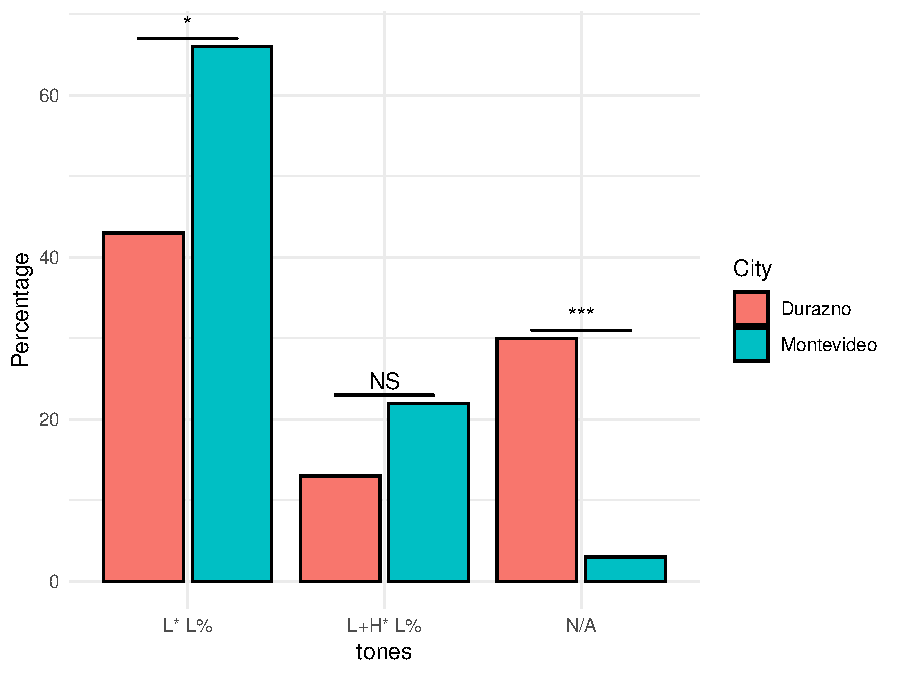
\includegraphics{main_files/figure-latex/unnamed-chunk-3-1.pdf}

\begin{longtable}[]{@{}lrr@{}}
\caption{\label{tab:unnamed-chunk-4}Table 1: Total percentage of each pitch accent in nuclear position for Broad Focus Decaratives.}\tabularnewline
\toprule\noalign{}
tones & Montevideo & Durazno \\
\midrule\noalign{}
\endfirsthead
\toprule\noalign{}
tones & Montevideo & Durazno \\
\midrule\noalign{}
\endhead
\bottomrule\noalign{}
\endlastfoot
!H* !H\% & 1 & 0 \\
H+L *L\% & 1 & 0 \\
H+L* L\% & 1 & 3 \\
L* !H\% & 1 & 0 \\
L* L\% & 66 & 43 \\
L+\textless H* L\% & 0 & 2 \\
L+H* !H\% & 0 & 2 \\
L+H* L!H\% & 0 & 3 \\
L+H* L\% & 22 & 13 \\
L+H* L* & 0 & 2 \\
L+H*+L L\% & 2 & 0 \\
L+¡H* L\% & 2 & 2 \\
NA & 3 & 30 \\
\end{longtable}

\begin{longtable}[]{@{}lrr@{}}
\caption{\label{tab:unnamed-chunk-5}Table 2: Total percentage of each pitch accent in nuclear position in which one group had produced it atleast 5 percent of the time in the data for Broad Focus Decaratives.}\tabularnewline
\toprule\noalign{}
tones & Montevideo & Durazno \\
\midrule\noalign{}
\endfirsthead
\toprule\noalign{}
tones & Montevideo & Durazno \\
\midrule\noalign{}
\endhead
\bottomrule\noalign{}
\endlastfoot
L* L\% & 66 & 43 \\
L+H* L\% & 22 & 13 \\
NA & 3 & 30 \\
\end{longtable}

\begin{quote}
In BFD we could mostly ignore boundary tones (e.g., L- and L\%)''
\end{quote}

We can integrate these if you prefer, but there does not look like there would be a major shift in the trend. If we need to recode things, it would be easiest for me with a list in an excel format, where one column is the original coding and the other is the simplified version. If I get one comprehensive list I can apply it to all data points and even tweak the recoding if it's needed later on.

\emph{Narrow Focus Declaratives}

\begin{longtable}[]{@{}lrr@{}}
\caption{\label{tab:unnamed-chunk-6}Table 3: Total percentage of each pitch accent in nuclear position for Narrow Focus Decaratives.}\tabularnewline
\toprule\noalign{}
tones & Montevideo & Durazno \\
\midrule\noalign{}
\endfirsthead
\toprule\noalign{}
tones & Montevideo & Durazno \\
\midrule\noalign{}
\endhead
\bottomrule\noalign{}
\endlastfoot
!H* L\% & 1 & 0 \\
H+L* L\% & 5 & 4 \\
L L\% & 1 & 0 \\
L* L\% & 25 & 28 \\
L+!H* L\% & 1 & 1 \\
L+!H*+L L\% & 2 & 2 \\
L+H* & 0 & 1 \\
L+H* !H\% & 3 & 12 \\
L+H* L\% & 23 & 32 \\
L+H* L\% & 1 & 0 \\
L+H*+L H\% & 1 & 0 \\
L+H*+L L\% & 17 & 3 \\
L+H*L\% & 0 & 1 \\
L+¡H L\% & 0 & 1 \\
L+¡H* !H\% & 1 & 1 \\
L+¡H* H\% & 0 & 1 \\
L+¡H* L\% & 13 & 7 \\
L+¡H*+L L\% & 4 & 1 \\
L+¡H*+L LH\% & 1 & 0 \\
L+¡H*L\% & 1 & 0 \\
¡H+L* L\% & 1 & 0 \\
NA & 1 & 5 \\
\end{longtable}

\textbf{Figure 2: Narrow Focus Declaratives in position N1 filtered}
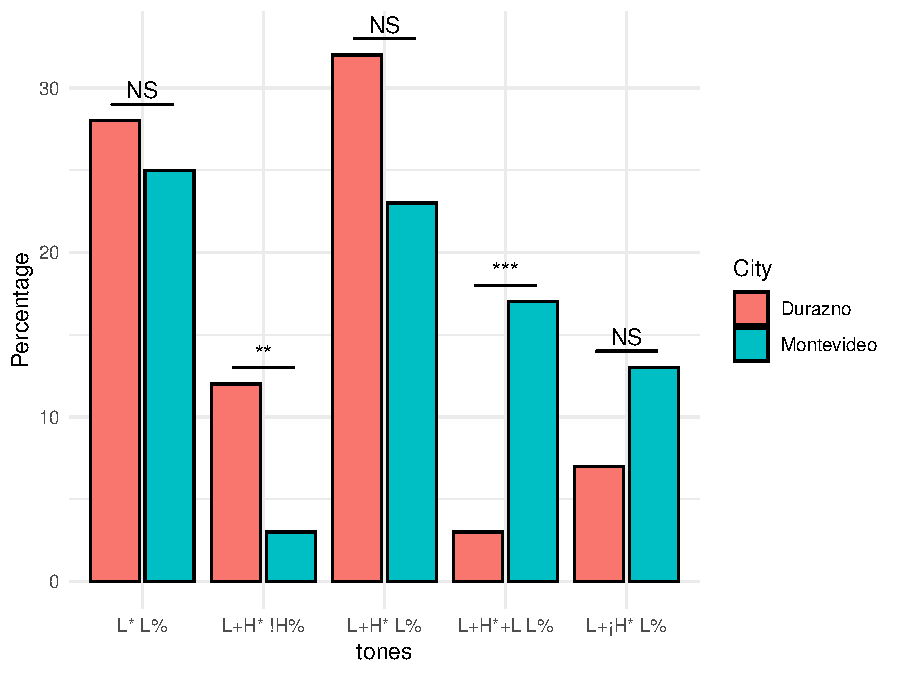
\includegraphics{main_files/figure-latex/unnamed-chunk-7-1.pdf}

\begin{longtable}[]{@{}lrr@{}}
\caption{\label{tab:unnamed-chunk-8}Table 4: Total percentage of each pitch accent in nuclear position in which one group had produced it atleast 5 percent of the time in the data for Narrow Focus Decaratives.}\tabularnewline
\toprule\noalign{}
tones & Montevideo & Durazno \\
\midrule\noalign{}
\endfirsthead
\toprule\noalign{}
tones & Montevideo & Durazno \\
\midrule\noalign{}
\endhead
\bottomrule\noalign{}
\endlastfoot
L* L\% & 25 & 28 \\
L+H* !H\% & 3 & 12 \\
L+H* L\% & 23 & 32 \\
L+H*+L L\% & 17 & 3 \\
L+¡H* L\% & 13 & 7 \\
\end{longtable}

\hypertarget{in-the-nfd-it-becomes-clear-that-the-h-ip-boundary-tone-is-a-clear-difference-between-dz-which-has-it-and-mv-that-mostly-doesnt.}{%
\subsection{In the NFD it becomes clear that the !H\% IP boundary tone is a clear difference between DZ (which has it) and MV (that mostly doesnt).''}\label{in-the-nfd-it-becomes-clear-that-the-h-ip-boundary-tone-is-a-clear-difference-between-dz-which-has-it-and-mv-that-mostly-doesnt.}}

There is a significant difference here (p \textless{} .005).

\hypertarget{at-the-same-time-we-see-that-the-tritonal-lhl-is-more-common-in-mv-than-dz.}{%
\subsection{At the same time we see that the tritonal L+H*+L is more common in MV than DZ.}\label{at-the-same-time-we-see-that-the-tritonal-lhl-is-more-common-in-mv-than-dz.}}

This is descriptively true (the count for MV is higher), but the poisson regression was not significant in this case (p \textgreater{} .05). This does not mean the difference is not real, but more likely that there just isn't enough data for the model to return a significant effect.

\hypertarget{lh-is-more-common-in-dz-than-mv.}{%
\subsection{L*+H is more common in DZ than MV.}\label{lh-is-more-common-in-dz-than-mv.}}

I don't actually see this in the data.

\hypertarget{what-seems-clear-in-both-dz-and-mv-is-that-upstepping-is-a-big-part-of-marking-focus-thus-in-an-utterance-full-of-lh-focus-is-rightly-marked-with-lh-in-cases-such-as-nfd5-con-manuel-these-are-all-high-peaks-but-due-to-the-lack-of-an-earlier-comparative-peak-they-are-not-classified-as-upstepped.}{%
\subsection{\texorpdfstring{What seems clear in both DZ and MV is that upstepping (¡) is a big part of marking focus, thus in an utterance full of L+H\emph{, focus is rightly marked with L+¡H}, in cases such as NFD5 Con Manuel, these are all high peaks but due to the lack of an earlier comparative peak they are not classified as upstepped.}{What seems clear in both DZ and MV is that upstepping (¡) is a big part of marking focus, thus in an utterance full of L+H, focus is rightly marked with L+¡H, in cases such as NFD5 Con Manuel, these are all high peaks but due to the lack of an earlier comparative peak they are not classified as upstepped.}}\label{what-seems-clear-in-both-dz-and-mv-is-that-upstepping-is-a-big-part-of-marking-focus-thus-in-an-utterance-full-of-lh-focus-is-rightly-marked-with-lh-in-cases-such-as-nfd5-con-manuel-these-are-all-high-peaks-but-due-to-the-lack-of-an-earlier-comparative-peak-they-are-not-classified-as-upstepped.}}

Here's a plot showing both cities productions for NFD5. It looks like the two groups are a little different than you've described above: Durazno speakers prefer L+H* !H\%. The Montevideo group, on the other hand, produce L+H*+L L\% the most.

\begin{longtable}[]{@{}lrr@{}}
\caption{\label{tab:unnamed-chunk-9}Table 5: Total percentage of each pitch accent in NFD5 `con Manuel'}\tabularnewline
\toprule\noalign{}
tones & Durazno & Montevideo \\
\midrule\noalign{}
\endfirsthead
\toprule\noalign{}
tones & Durazno & Montevideo \\
\midrule\noalign{}
\endhead
\bottomrule\noalign{}
\endlastfoot
H+L* L\% & 5 & 0 \\
L+!H*+L L\% & 5 & 0 \\
L+H* !H\% & 60 & 20 \\
L+H* L\% & 10 & 27 \\
L+H*+L L\% & 10 & 53 \\
L+¡H* !H\% & 5 & 0 \\
NA & 5 & 0 \\
\end{longtable}

\begin{longtable}[]{@{}lrr@{}}
\caption{\label{tab:unnamed-chunk-10}Table 6: Total percentage of each pitch accent in NFD5 `con Manuel' occuring at least 5 total times}\tabularnewline
\toprule\noalign{}
tones & Durazno & Montevideo \\
\midrule\noalign{}
\endfirsthead
\toprule\noalign{}
tones & Durazno & Montevideo \\
\midrule\noalign{}
\endhead
\bottomrule\noalign{}
\endlastfoot
L+H* !H\% & 60 & 20 \\
L+H* L\% & 10 & 27 \\
L+H*+L L\% & 10 & 53 \\
\end{longtable}

\textbf{Figure 3: Total percentage of each pitch accent in NFD5 `con Manuel' occuring at least 5 total times}
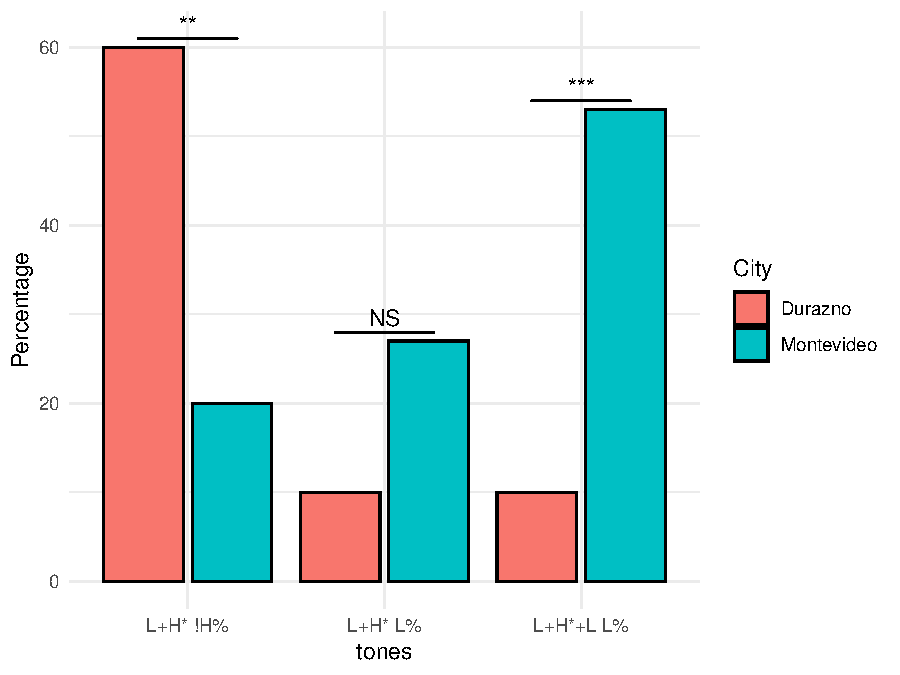
\includegraphics{main_files/figure-latex/unnamed-chunk-11-1.pdf}

\hypertarget{thus-if-in-the-count-for-focalized-items-lh-rather-than-lh-it-should-be-undestood-that-these-are-in-such-a-case-not-different-and-can-be-grouped-whereas-in-sentences-with-pn-peaks-these-are-different.}{%
\subsection{Thus if in the count for focalized items L+H* rather than L+¡H* it should be undestood that these are, in such a case not different and can be grouped, whereas in sentences with PN peaks these are different.}\label{thus-if-in-the-count-for-focalized-items-lh-rather-than-lh-it-should-be-undestood-that-these-are-in-such-a-case-not-different-and-can-be-grouped-whereas-in-sentences-with-pn-peaks-these-are-different.}}

As above, a full list of these cases would be ideal if we need to re-code some things.

\hypertarget{socially-at-least-before-the-current-updated-data-women-tended-to-use-the-tritonal-lhl-as-well-as-the-upstep-more-than-men-this-again-is-a-key-distinction-as-it-once-again-provided-evidence-for-the-theory-of-females-making-greater-contrasts-and-therfore-greater-clarity-in-speaking.}{%
\subsection{Socially, (at least before the current updated data) women tended to use the tritonal L+H*+L as well as the upstep ¡ more than men, this again is a key distinction as it once again provided evidence for the theory of females making greater contrasts and therfore greater clarity in speaking.}\label{socially-at-least-before-the-current-updated-data-women-tended-to-use-the-tritonal-lhl-as-well-as-the-upstep-more-than-men-this-again-is-a-key-distinction-as-it-once-again-provided-evidence-for-the-theory-of-females-making-greater-contrasts-and-therfore-greater-clarity-in-speaking.}}

Here's some visualizations of sex, if these look good, I can also run inferential statistics for the comparisons of interest.

\textbf{Figure 4: Total percentage of each pitch accent by sex in each city in narrow focus declaratives and the N1 position}
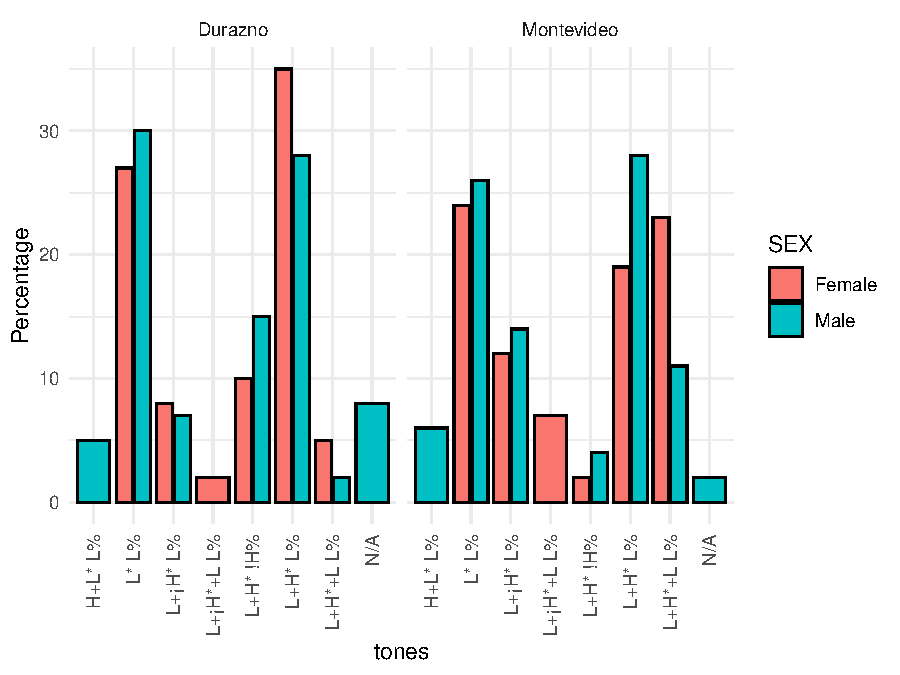
\includegraphics{main_files/figure-latex/unnamed-chunk-12-1.pdf}

\textbf{Figure 5: Total percentage of each pitch accent by sex in each city in broad focus declaratives and the N position}
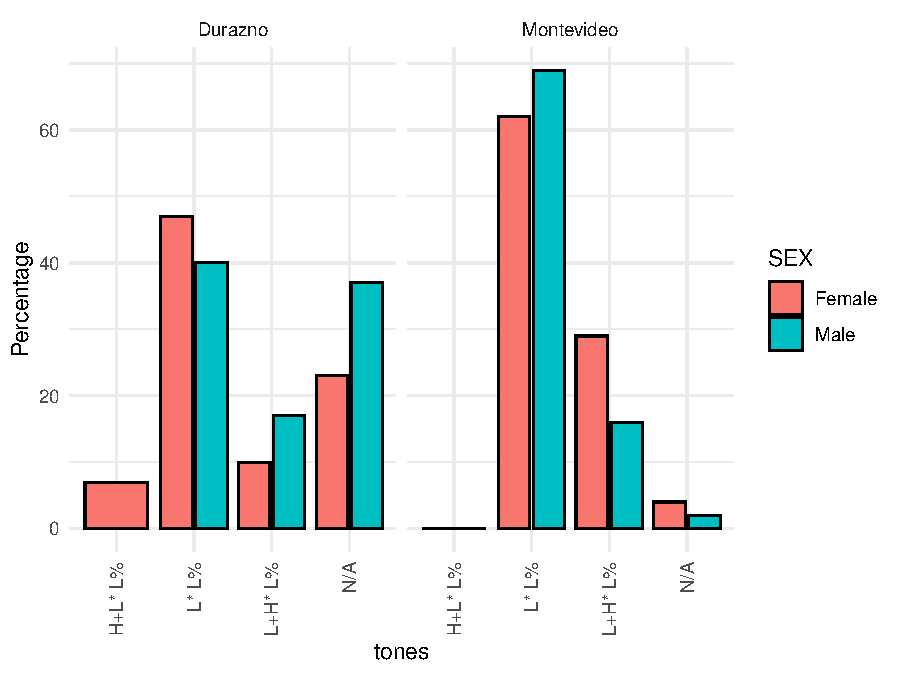
\includegraphics{main_files/figure-latex/unnamed-chunk-13-1.pdf}

\hypertarget{also-if-you-find-that-certain-utterance-tend-to-prefer-unique-forms-such-as-nfd5-a-statement-of-the-obvious-where-tritonals-may-be-more-common-or-where-the-mid-boundary-tone-h-is-more-frequent-this-is-also-of-note.}{%
\subsection{Also if you find that certain utterance tend to prefer unique forms, such as NFD5 ``a statement of the obvious'' where tritonals may be more common or where the mid-boundary tone !H\% is more frequent this is also of note.}\label{also-if-you-find-that-certain-utterance-tend-to-prefer-unique-forms-such-as-nfd5-a-statement-of-the-obvious-where-tritonals-may-be-more-common-or-where-the-mid-boundary-tone-h-is-more-frequent-this-is-also-of-note.}}

These tables and figures show the percentage of each pitch accent in each item for both broad and narrow focus declaratives. Again, everything is ``N'' or ``N1'' in terms of position.

\textbf{Figure 6: Total percentage of each pitch accent for narrow focus declaratives in each item per city}
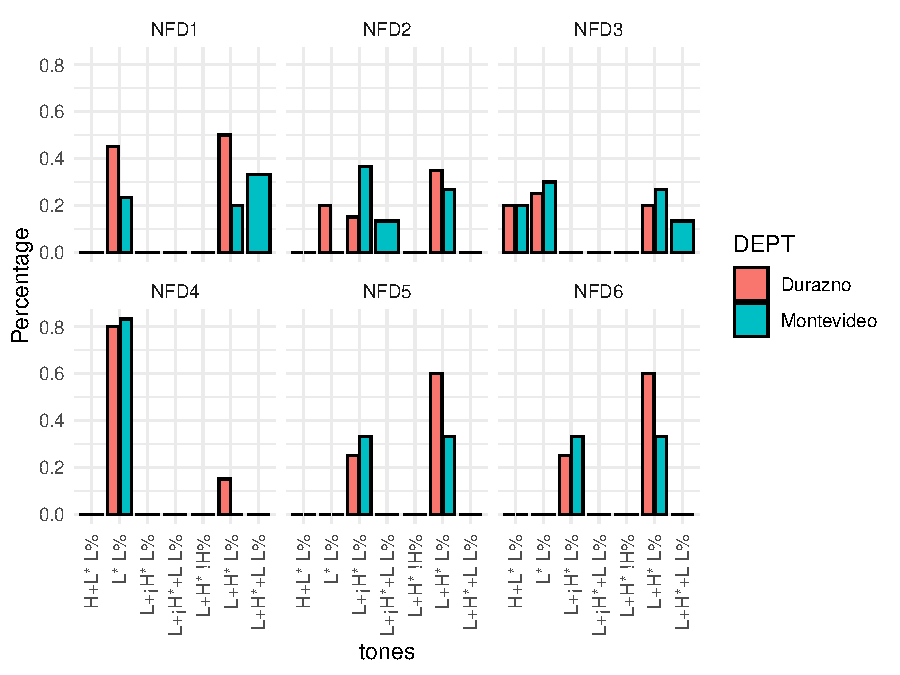
\includegraphics{main_files/figure-latex/unnamed-chunk-14-1.pdf}

\begin{longtable}[]{@{}lllr@{}}
\caption{\label{tab:unnamed-chunk-15}Table 7: Total percentage of each pitch accent for narrow focus declaratives in each item per city}\tabularnewline
\toprule\noalign{}
tones & DEPT & Sentence & Percentage \\
\midrule\noalign{}
\endfirsthead
\toprule\noalign{}
tones & DEPT & Sentence & Percentage \\
\midrule\noalign{}
\endhead
\bottomrule\noalign{}
\endlastfoot
H+L* L\% & Durazno & NFD3 & 0.2000000 \\
H+L* L\% & Durazno & NFD1 & 0.0000000 \\
H+L* L\% & Durazno & NFD2 & 0.0000000 \\
H+L* L\% & Durazno & NFD4 & 0.0000000 \\
H+L* L\% & Durazno & NFD5 & 0.0000000 \\
H+L* L\% & Durazno & NFD6 & 0.0000000 \\
H+L* L\% & Montevideo & NFD3 & 0.2000000 \\
H+L* L\% & Montevideo & NFD1 & 0.0000000 \\
H+L* L\% & Montevideo & NFD2 & 0.0000000 \\
H+L* L\% & Montevideo & NFD4 & 0.0000000 \\
H+L* L\% & Montevideo & NFD5 & 0.0000000 \\
H+L* L\% & Montevideo & NFD6 & 0.0000000 \\
L* L\% & Durazno & NFD3 & 0.2500000 \\
L* L\% & Durazno & NFD1 & 0.4500000 \\
L* L\% & Durazno & NFD2 & 0.2000000 \\
L* L\% & Durazno & NFD4 & 0.8000000 \\
L* L\% & Durazno & NFD5 & 0.0000000 \\
L* L\% & Durazno & NFD6 & 0.0000000 \\
L* L\% & Montevideo & NFD3 & 0.3000000 \\
L* L\% & Montevideo & NFD1 & 0.2333333 \\
L* L\% & Montevideo & NFD2 & 0.0000000 \\
L* L\% & Montevideo & NFD4 & 0.8333333 \\
L* L\% & Montevideo & NFD5 & 0.0000000 \\
L* L\% & Montevideo & NFD6 & 0.0000000 \\
L+H* !H\% & Durazno & NFD3 & 0.0000000 \\
L+H* !H\% & Durazno & NFD1 & 0.0000000 \\
L+H* !H\% & Durazno & NFD2 & 0.0000000 \\
L+H* !H\% & Durazno & NFD4 & 0.0000000 \\
L+H* !H\% & Durazno & NFD5 & 0.0000000 \\
L+H* !H\% & Durazno & NFD6 & 0.0000000 \\
L+H* !H\% & Montevideo & NFD3 & 0.0000000 \\
L+H* !H\% & Montevideo & NFD1 & 0.0000000 \\
L+H* !H\% & Montevideo & NFD2 & 0.0000000 \\
L+H* !H\% & Montevideo & NFD4 & 0.0000000 \\
L+H* !H\% & Montevideo & NFD5 & 0.0000000 \\
L+H* !H\% & Montevideo & NFD6 & 0.0000000 \\
L+H* L\% & Durazno & NFD3 & 0.2000000 \\
L+H* L\% & Durazno & NFD1 & 0.5000000 \\
L+H* L\% & Durazno & NFD2 & 0.3500000 \\
L+H* L\% & Durazno & NFD4 & 0.1500000 \\
L+H* L\% & Durazno & NFD5 & 0.6000000 \\
L+H* L\% & Durazno & NFD6 & 0.6000000 \\
L+H* L\% & Montevideo & NFD3 & 0.2666667 \\
L+H* L\% & Montevideo & NFD1 & 0.2000000 \\
L+H* L\% & Montevideo & NFD2 & 0.2666667 \\
L+H* L\% & Montevideo & NFD4 & 0.0000000 \\
L+H* L\% & Montevideo & NFD5 & 0.3333333 \\
L+H* L\% & Montevideo & NFD6 & 0.3333333 \\
L+H*+L L\% & Montevideo & NFD3 & 0.1333333 \\
L+H*+L L\% & Montevideo & NFD1 & 0.3333333 \\
L+H*+L L\% & Montevideo & NFD2 & 0.0000000 \\
L+H*+L L\% & Montevideo & NFD4 & 0.0000000 \\
L+H*+L L\% & Montevideo & NFD5 & 0.0000000 \\
L+H*+L L\% & Montevideo & NFD6 & 0.0000000 \\
L+¡H* L\% & Durazno & NFD3 & 0.0000000 \\
L+¡H* L\% & Durazno & NFD1 & 0.0000000 \\
L+¡H* L\% & Durazno & NFD2 & 0.1500000 \\
L+¡H* L\% & Durazno & NFD4 & 0.0000000 \\
L+¡H* L\% & Durazno & NFD5 & 0.2500000 \\
L+¡H* L\% & Durazno & NFD6 & 0.2500000 \\
L+¡H* L\% & Montevideo & NFD3 & 0.0000000 \\
L+¡H* L\% & Montevideo & NFD1 & 0.0000000 \\
L+¡H* L\% & Montevideo & NFD2 & 0.3666667 \\
L+¡H* L\% & Montevideo & NFD4 & 0.0000000 \\
L+¡H* L\% & Montevideo & NFD5 & 0.3333333 \\
L+¡H* L\% & Montevideo & NFD6 & 0.3333333 \\
L+¡H*+L L\% & Montevideo & NFD3 & 0.0000000 \\
L+¡H*+L L\% & Montevideo & NFD1 & 0.0000000 \\
L+¡H*+L L\% & Montevideo & NFD2 & 0.1333333 \\
L+¡H*+L L\% & Montevideo & NFD4 & 0.0000000 \\
L+¡H*+L L\% & Montevideo & NFD5 & 0.0000000 \\
L+¡H*+L L\% & Montevideo & NFD6 & 0.0000000 \\
\end{longtable}

\textbf{Figure 7: Total percentage of each pitch accent for broad focus declaratives in each item per city}
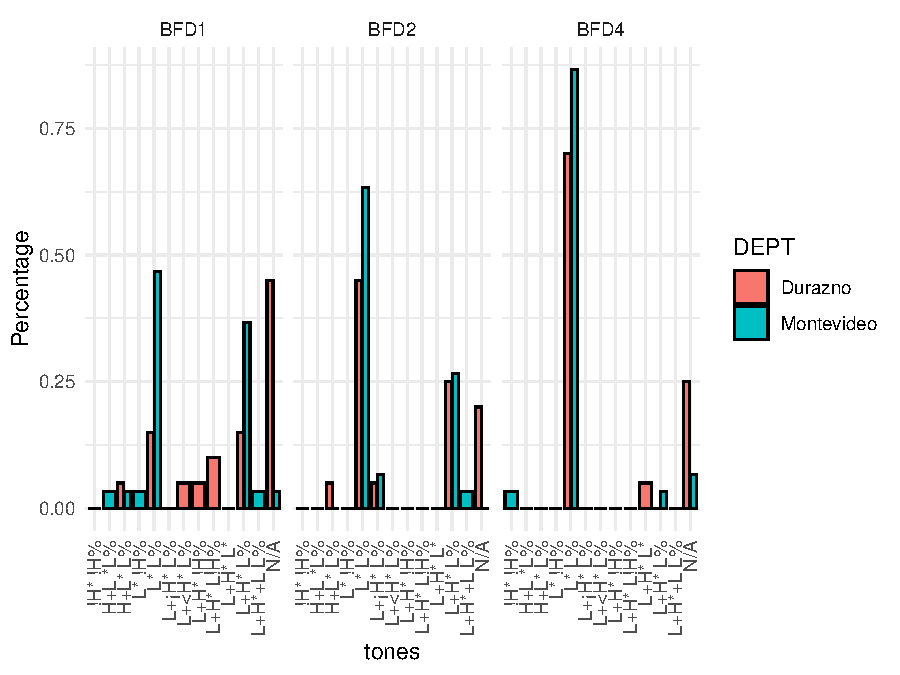
\includegraphics{main_files/figure-latex/unnamed-chunk-16-1.pdf}

\begin{longtable}[]{@{}lllr@{}}
\caption{\label{tab:unnamed-chunk-17}Table 8: Total percentage of each pitch accent for broad focus declaratives in each item per city}\tabularnewline
\toprule\noalign{}
tones & DEPT & Sentence & Percentage \\
\midrule\noalign{}
\endfirsthead
\toprule\noalign{}
tones & DEPT & Sentence & Percentage \\
\midrule\noalign{}
\endhead
\bottomrule\noalign{}
\endlastfoot
!H* !H\% & Montevideo & BFD4 & 0.0333333 \\
!H* !H\% & Montevideo & BFD1 & 0.0000000 \\
!H* !H\% & Montevideo & BFD2 & 0.0000000 \\
H+L *L\% & Montevideo & BFD4 & 0.0000000 \\
H+L *L\% & Montevideo & BFD1 & 0.0333333 \\
H+L *L\% & Montevideo & BFD2 & 0.0000000 \\
H+L* L\% & Durazno & BFD4 & 0.0000000 \\
H+L* L\% & Durazno & BFD1 & 0.0500000 \\
H+L* L\% & Durazno & BFD2 & 0.0500000 \\
H+L* L\% & Montevideo & BFD4 & 0.0000000 \\
H+L* L\% & Montevideo & BFD1 & 0.0333333 \\
H+L* L\% & Montevideo & BFD2 & 0.0000000 \\
L* !H\% & Montevideo & BFD4 & 0.0000000 \\
L* !H\% & Montevideo & BFD1 & 0.0333333 \\
L* !H\% & Montevideo & BFD2 & 0.0000000 \\
L* L\% & Durazno & BFD4 & 0.7000000 \\
L* L\% & Durazno & BFD1 & 0.1500000 \\
L* L\% & Durazno & BFD2 & 0.4500000 \\
L* L\% & Montevideo & BFD4 & 0.8666667 \\
L* L\% & Montevideo & BFD1 & 0.4666667 \\
L* L\% & Montevideo & BFD2 & 0.6333333 \\
L+\textless H* L\% & Durazno & BFD4 & 0.0000000 \\
L+\textless H* L\% & Durazno & BFD1 & 0.0500000 \\
L+\textless H* L\% & Durazno & BFD2 & 0.0000000 \\
L+H* !H\% & Durazno & BFD4 & 0.0000000 \\
L+H* !H\% & Durazno & BFD1 & 0.0500000 \\
L+H* !H\% & Durazno & BFD2 & 0.0000000 \\
L+H* L!H\% & Durazno & BFD4 & 0.0000000 \\
L+H* L!H\% & Durazno & BFD1 & 0.1000000 \\
L+H* L!H\% & Durazno & BFD2 & 0.0000000 \\
L+H* L\% & Durazno & BFD4 & 0.0000000 \\
L+H* L\% & Durazno & BFD1 & 0.1500000 \\
L+H* L\% & Durazno & BFD2 & 0.2500000 \\
L+H* L\% & Montevideo & BFD4 & 0.0333333 \\
L+H* L\% & Montevideo & BFD1 & 0.3666667 \\
L+H* L\% & Montevideo & BFD2 & 0.2666667 \\
L+H* L* & Durazno & BFD4 & 0.0500000 \\
L+H* L* & Durazno & BFD1 & 0.0000000 \\
L+H* L* & Durazno & BFD2 & 0.0000000 \\
L+H*+L L\% & Montevideo & BFD4 & 0.0000000 \\
L+H*+L L\% & Montevideo & BFD1 & 0.0333333 \\
L+H*+L L\% & Montevideo & BFD2 & 0.0333333 \\
L+¡H* L\% & Durazno & BFD4 & 0.0000000 \\
L+¡H* L\% & Durazno & BFD1 & 0.0000000 \\
L+¡H* L\% & Durazno & BFD2 & 0.0500000 \\
L+¡H* L\% & Montevideo & BFD4 & 0.0000000 \\
L+¡H* L\% & Montevideo & BFD1 & 0.0000000 \\
L+¡H* L\% & Montevideo & BFD2 & 0.0666667 \\
N/A & Durazno & BFD4 & 0.2500000 \\
N/A & Durazno & BFD1 & 0.4500000 \\
N/A & Durazno & BFD2 & 0.2000000 \\
N/A & Montevideo & BFD4 & 0.0666667 \\
N/A & Montevideo & BFD1 & 0.0333333 \\
N/A & Montevideo & BFD2 & 0.0000000 \\
\end{longtable}


\end{document}
